%!TEX root = cscw2018-comic.tex
\subsection{Memorability, Social Proof and Framing}
Approaches to make a message more attractive and persuasive has long been a focus for a variety of different fields including computational linguistic, social networking, and advertising \cite{smith1996message,tversky1981framing,danescu2012you,huntertowards,maheswaran1990influence,grewal1994moderating}. Well established research provides three major factors in constructing persuasive messages, memorability, social proof and message framing.

\begin{description}
\item[Memorability]
The most simple but effective way to achieve successful and long-last persuasion is through memorability.In \cite{danescu2012you} the study showed that using unusual word choices and more general theme makes it easier to connect with reader's daily life and makes the message more memorable. Through the use of unexpected words and phrases, the message is more likely to capture reader's attention compared text using normal phrases. And the theme should be as general as possible to help readers connect with the message, so it can stay in the reader's mind longer.

\item[Social Proof]
Implying social norm through the message is another persuasive technique.  Goldstein et. al conducted an interest experiment in the hotel on motivating environmental conservation. They found employing descriptive norms (e.g., "the majority of guests reuse their towels") has more persuasive power than solely mentioning environmental protection. And this normative message gets more persuasiveness when the described setting is closer to individuals' immediate situational circumstances (e.g., "the majority of guests in this room reuse their towels") \cite{goldstein2008room}.

\item[Message Framing]
Among these tactics, message framing is one of the most basic and intuitive methods to generate memorable and persuasive messages \cite{smith1996message,tversky1981framing}. This is mainly because message framing and phrasing generally doesn't require additional information or data visualization. Its simplicity contributes to the various researches on the effect of message framing in memorability. Tversky and Kahneman found using different reference point to frame the same sentence can result in reader's different response\cite{tversky1992advances,tversky1981framing,kahneman1984choices}.It shows that variations of reference point of a decision can determine whether the reader will evaluate it as a gain or a loss, thus changing their decision. For example, choices involving gains are often risk averse and choices involving losses are often risk taking.

\end{description}
All those techniques are essential for our design of messages to persuade behavioral change. However, little is known for persuading people in form of comics which leads the first research question. RQ1: Are same persuasive techniques can also be used in comic persuasion?

\subsection{Persuade beyond text}
Previous research shows using visual representations are more attractive to readers comparing to text messages \cite{selker2015sweetbuildinggreeter,consolvo2008activity}. Selker et al. retrieves motivational images from 9GAG, Google, with energy-saving messages, to motivate people's energy saving behaviors and found those comics has higher persuasive power comparing to plain text \cite{selker2015sweetbuildinggreeter}. Consolvo et. al built Ubifit Garden that successfully encourage physical activity by present user's exercise data as different elements in a garden \cite{consolvo2008activity}.

Persuasive message in a visual form can raise persuadee's awareness and have a greater chance to persuade change. However, as a common visual form, no one has looked at the perceived persuasiveness of comics.

RQ2: Does a persuasive message in the comic form is perceived as more persuasive?

\subsection{Comics Elements}
\begin{figure}
  \centering
  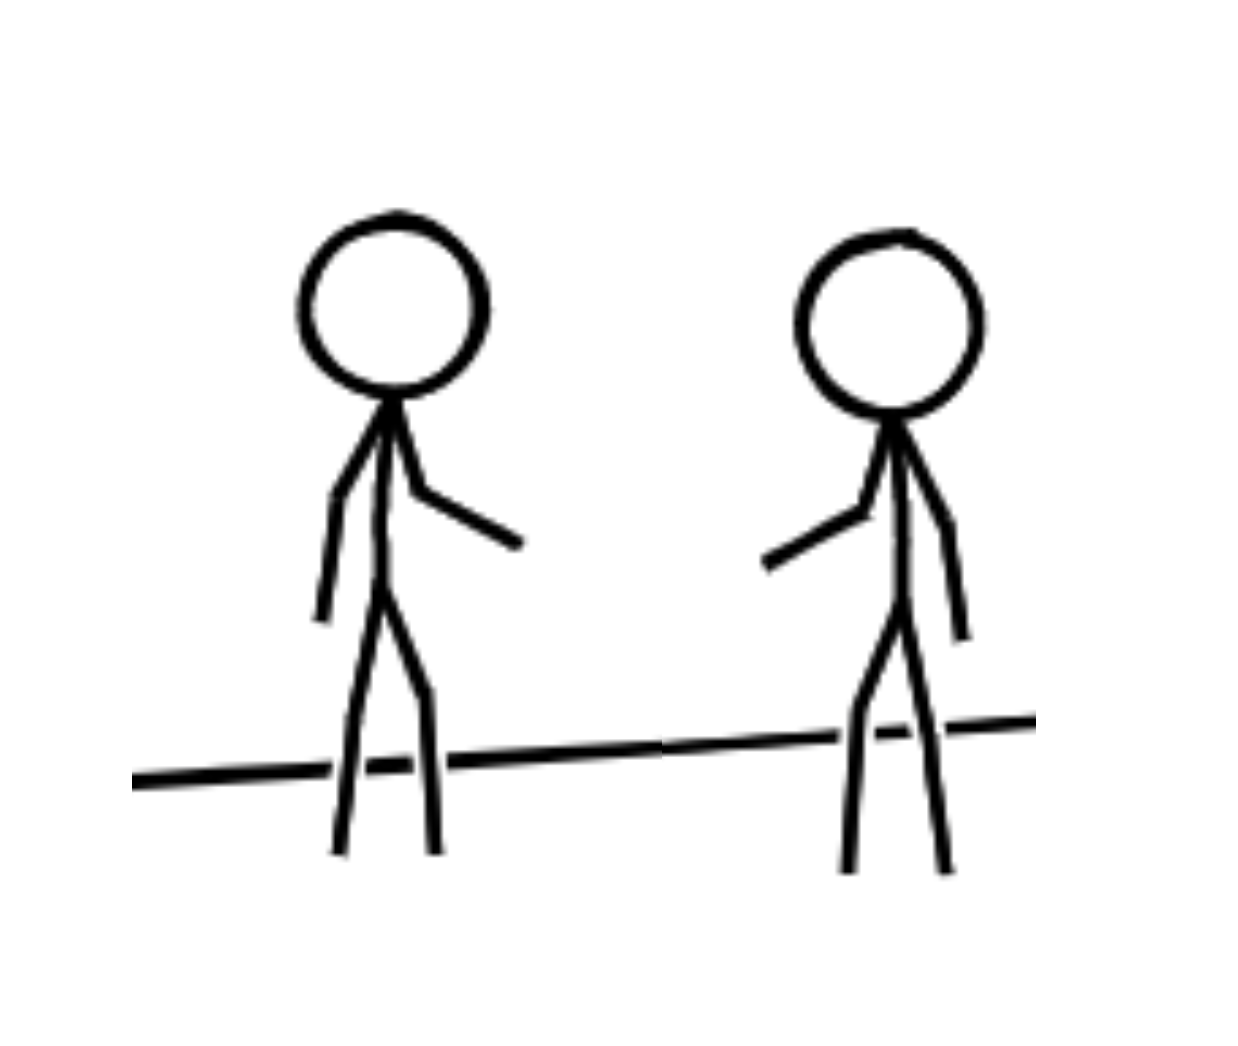
\includegraphics[width=0.3\columnwidth]{figures/xkcd_example}
  \caption{A example of abstract comic figure in XKCD style}
  \label{fig:xkcd}
\end{figure}

As a form of art, the creation of comics has few limitation. Although there is no common template that could describe all comics, if we take a closer look at each comic, it is not hard to see that every comic consists of several fundamental components. We categorize comic elements into four key groups: 1) characters, 2) character gestures, 3) background shading 4) text bubble. To represent a persuasive message in comic form, we need to determine each of those four parameters.

As Scott McCloud mentioned in his book, the reader is more likely to project him/herself onto the character in the comic when the comic getting abstract \cite{scott1993understanding}. By taking the perspective of the character, the reader will internalize the information his/her character trying to express or receive. If the information is persuasive, the internalization will imply a higher chance of expected behavior change. Therefore, in this study, we choose to use an abstract yet well-recognized comic style, the xkcd style created by Randall Munroe, in our generated persuasive comic messages \cite{munroe2009xkcd},see Figure~\ref{fig:xkcd}.

Beside the abstractness of the character, the relationship between characters is also important. In real world, previous research suggests that messages are more persuasive if the person communicating the ideas is someone the receiver relates \cite{daddis2008influence,merga2014peer,shin2013user}. People are more likely to be influenced by their close friends than strangers. In abstract comics, the relationship between characters is usually modeled by the distance between characters \cite{scott1993understanding}. So, it is reasonable to believe the link still holds in the world of comics as the reader tends to project his/herself onto the character.

The gesture of a character is another important component in the comic. The gesture of a character can help reader to understand what happens and the emotion of the character. Different gestures also imply the intensity of an emotion. As a common technique, cartoonists often use the gesture to intensify the feeling that they want to express to the reader. For a persuasive message, the intensified emotion may make the message more memorable than a plain tone. Thus, in this study, the gesture is another key element that we believe may moderate the effectiveness of a comic message.

A rich body of research has demonstrated the relationship between background shading and the emotion in comics \cite{scott1993understanding}. Align with the idea of increasing memorability, representations with strong emotion can make the message more unique.

The word bubble is the most common place in comics to incorporate text information. In a persuasive comic, the word bubble expresses the text content of the message.

RQ3: Does different elements in a persuasive comic affect its perceived persuasiveness?
